\subsection{Staying Organised}
So far our examples have been extremely short, but imagine having dozens of chapters with dozens of packages and whatever configuration is necessary for them.
One thing we can do is split up our document into the \emph{preamble}, the file \verb|main.tex|, where we have all the setup, and the \emph{content}.
The content can be split up whichever way you see fit --- with the more complicated it is, the more you would want to split it up. 

Let's expand our working directory like seen below. You can also just copy the files from \verb|Example2| .
\clearpage
\begin{verbatim}
Example2
├── bibliography.bib
├── main.pdf
├── main.tex
├── code
│   └── code.m
├── figures
│   └── gradient-circle.png
└── files
    ├── introduction.tex
    ├── animal-rights.tex
    └── animal-lefts.tex
\end{verbatim}

Let's first take a look at our preamble file, \verb|main.tex|.

\lstinputlisting[language=tex, caption={\texttt{main.tex}}]{files/lesson-plan/getting-started/Example2/example.tex}

\verb|\usepackage{geometry}| and its command \verb|\geometry{}| allows us to set each margin individually.
APA styling suggests 1 inch all around, but you may need to adjust the left margin for binding a thesis.

The package \verb|setspace| and its command \verb|\doublespacing| provides automatic double spacing.

The package \verb|listings| allows presenting code in the exact way it is seen in this document. We will discuss it more in the coming sections.

The \verb|tikz| package is what we use for mathematical drawing, graphing, importing pictures, and much more.
We will discuss it more in the coming sections.

To ``inject'' the contents of another file into our preamble, the \verb|import| package gives us \verb|\subimport{}{}|.
The first bracket requires a relative path starting from the root of your working directory, and the second bracket is the name of the file.
You can include a \verb|\subimport{}{}| in a file that has itself been \texttt{subimport}ed, and this is the key to organisation.

VSCode will help you navigate the folders and find the files.
As you star typing \verb|\subimport| it will offer the command as a suggestion.
Select it by pressing \verb|tab|, navigate to choose the folder called \verb|files/|, then press \verb|tab| to select.
Press \verb|tab| again to move to the second set of brackets. If it doesn't display options, press \verb|ctrl+space|, and you can pick the file.
\begin{figure}[h]
    \centering
    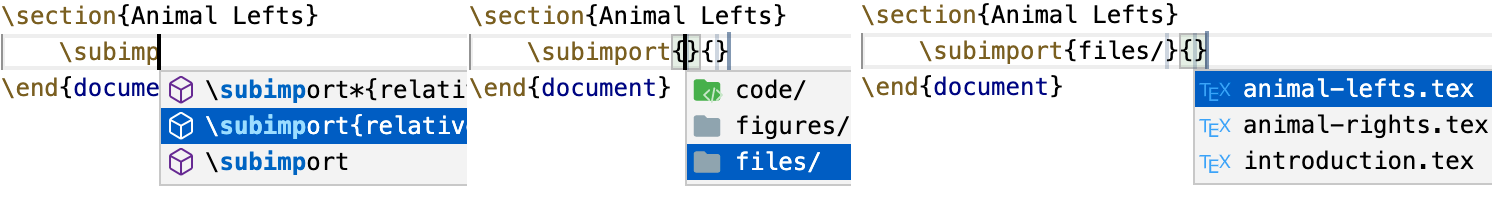
\includegraphics[width=\textwidth]{figures/subimport.png}
    \caption{Intellisense-assisted picking files.}
    \label{fig:animal-lefts}
\end{figure}

The biggest advantage of this separation is that each content file has absolutely no configuration at all.
This is called \emph{Separation of concerns}, and it allows us to just focus on the content, and all of the setting up comes from a template with minor tweaks.

\subsection{Figure and caption}
Our \verb|introduction.tex| file, then, looks like this:
\lstinputlisting[language=tex, caption={\texttt{introduction.tex}}]{files/lesson-plan/getting-started/Example2/files/introduction.tex}

With the output as seen in Figure \ref{fig:figures}

\begin{figure}[h]
    \centering
        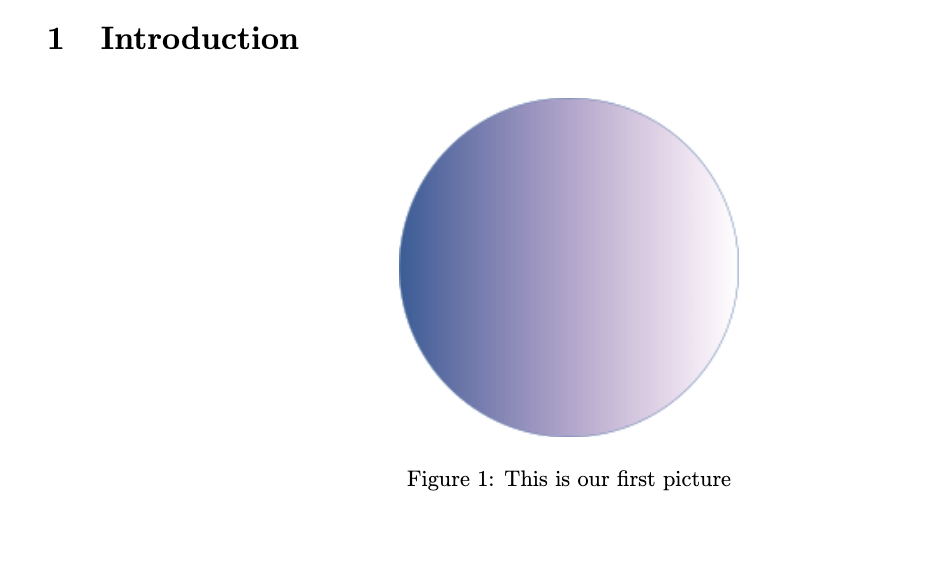
\includegraphics[width=0.7\textwidth]{figures/figures.png}
    \caption{Output from \texttt{introduction.tex}}
    \label{fig:figures}
\end{figure}

\verb|\begin{figure}...\end{figure}| creates a figure \emph{environment}.
\LaTeX\ tries to find the best position for every environment, but you can force their position by passing the option \verb|[h]|.
Usually contents are left-adjusted, so we can push the environment to the centre by using \verb|\centering|.
\verb|\caption{}| automatically numbers sequentially.

\verb|tikz| provides the \verb|\includegraphics{}| command that imports our picture.
Often we need to scale pictures, which can be achieved with the options \verb|width=0.5\textwidth| or \verb|scale=0.8|.
\verb|\textwidth| is a \LaTeX\ variable which automatically calculates the usable size of your document.
So in order to scale the picture to 0.5 of the textwidth, we would use:
\begin{lstlisting}
\includegraphics[width=0.5\textwidth]{figures/gradient-cicle.png}
\end{lstlisting}

\paragraph{Note: }
Occasionally weneed to put two pictures side-by-side. How would you achieve that? The simplest way is to include both within the same \verb|figure| environment and make sure their widths are less than half of the allowable text width: \verb|width=0.5\textwidth|.
If you need captions on each subfigure, then you are looking for the package \verb|subcaption|, and you can find more information \href{http://mirrors.ibiblio.org/CTAN/macros/latex/contrib/caption/subcaption.pdf}{here}.

\begin{lstlisting}{tex}
\begin{figure}[h]
\centering
    \includegraphics[width=0.49\textwidth]{figures/pic1.png}
    \includegraphics[width=0.49\textwidth]{figures/pic2.png}
\caption{Two pictures in one figure environment}
\label{fig:pic1-pic2}
\end{figure}
\end{lstlisting}   

\subsection{Label and cross-reference}
The \verb|\label{}| command is paired with \verb|\ref{}| for automatic cross-referencing across any file of our document.
From the \verb|animal-rights.tex| file we are able to reference both the table in this file and the figure in \verb|introduction.tex|.
This makes it important to be very explicit with our labels, so you can actually find them!
The suggestion is to use \verb|fig:file-name| for figures, \verb|eq:name| for equations, and so on.
With larger documents, you may even want to include chapter references to you can ``filter'' the names: \verb|fig:ch6:dog-with-tail|.

\lstinputlisting[language=tex, caption={\texttt{animal-rights.tex}}]{files/lesson-plan/getting-started/Example2/files/animal-rights.tex}
which looks like this:
\begin{figure}[h]
    \centering
        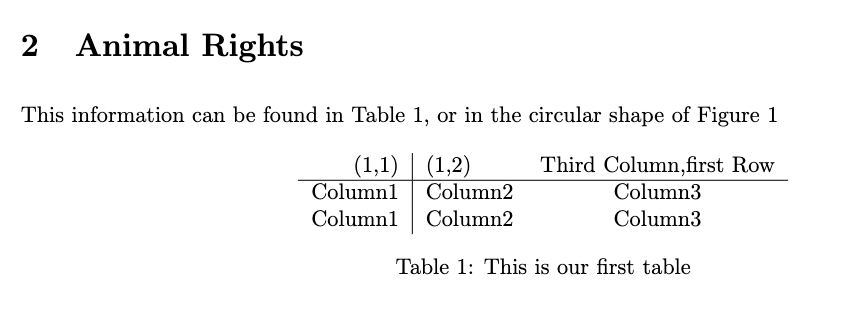
\includegraphics[width=0.8\textwidth]{figures/tables.png}
    \label{fig:tables}
\end{figure}

\subsection{Table}
\verb|\begin{table}...\end{table}| creates a table \emph{environment}, which is different from creating a table itself.
\verb|table| has similar properties to \verb|figure|, allowing you to set a caption, label and position.

\verb|tabular|, on the other hand, creates a table. This is always followed with curly brackets deciding the \textbf{number of columns}, the \textbf{adjustment} of the text and whether there are \textbf{vertical dividers}.
\verb!{r|lc}! means a right-adjusted column with a vertical divider, a left-adjusted column, and a centre-adjusted column.

Each column is separated by \verb|&| and each row is separated by \verb|\\|. \verb|\hline| is used to produce a horizontal line that separates titles from content.
\paragraph{Note:} As you may have noticed, some characters have special meaning, like \&, \{, \} and \textbackslash. To display the literal symbol, it needs to be \emph{escaped} by a preceeding \verb|\|, like this: \verb|\&|, \verb|\{|, etc. The backslash is an exception, because \verb|\\| is also a special character, so you have to use \verb|\textbackslash|.

\subsection{Lists}
There are two types of lists: numbered and unnumbered, and these are \verb|enumerate| and \verb|itemize| environments, respectively.
Take a look at the code in \verb|animal-lefts.tex|.

\lstinputlisting[language=tex, caption={animal-lefts.tex}]{files/lesson-plan/getting-started/Example2/files/animal-lefts.tex}

Resulting in:

\begin{figure}[h]
    \centering
        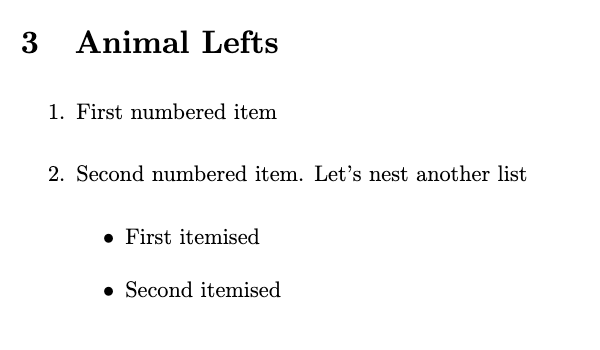
\includegraphics[scale=0.8]{figures/list.png}
    \label{fig:list}
\end{figure}

A new entry is only created with \verb|\item|, so you can have as much code between entries as you want, including other environments and nestings of \verb|enumerate|, like this:
\clearpage
\begin{lstlisting}
\begin{enumerate}
    \item First question
        \begin{enumerate}
            \item Sub question
                \begin{enumerate}
                    \item Item on subquestion
                \end{enumerate}
    \end{enumerate}
    \item Second question
\end{enumerate}
\end{lstlisting}
Resulting in:
\begin{figure}[h]
    \centering
        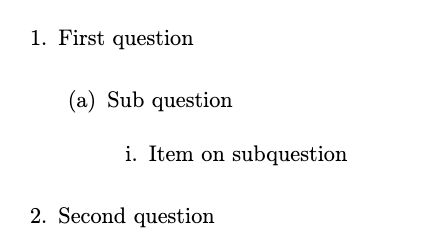
\includegraphics[]{figures/list-nested.png}
    \label{fig:list-nested}
\end{figure}

\subsection{Code}
As mentioned earlier, the package \verb|listings| creates an environment to present code in the exact way it is seen in this document.
The appearance of the frame can be changed greatly, and \texttt{listings} is very well documented \href{https://texdoc.org/serve/listings.pdf/0}{here}.
Generally, stick to the options presented in the preamble and in the templates, and it will cover most of your needs, namely:

\begin{lstlisting}
\lstset{
	numbers=left, frame=single, breaklines=true, %Keep text inside a frame, and number each line.
	basicstyle = \scriptsize\ttfamily, %smaller size, monospaced
}
\end{lstlisting}

If you are looking for highlighting in the same way you'd find in your editor, look for the package \texttt{minted}.
It requires a bit of setup, but you can find more information \href{http://tug.ctan.org/macros/latex/contrib/minted/minted.pdf}{here}.

We have the option of manually writing the code in-file with the \verb|lstlisting| environment.
Try writing in-file for yourself!
Tip: An environment is always \verb|\begin{environment-name}|\dots\verb|\end{environment-name}|.

It is also possible to import from another file with \verb|\lstinputlisting{}|, and you can see an example of it below.
Don't worry about remembering it exactly --- you will always be able to check documentation, the internet, or as we will describe at the end of this, use a \emph{snippet}.
Snippets are the key to typesetting documents incredibly fast, and will be covered extensively in the end.
   
\begin{lstlisting}
    \lstinputlisting[language=Matlab, caption={My Example code}, label={code:matrix}]{code/code.m}
\end{lstlisting}

\paragraph{Note:}
The \texttt{verbatim} environment, \verb!\verb||! and \verb|\texttt{}| produce monospaced fonts as well, and there are moments when each one is appropriate.
Generally \verb!\verb||! (which can also be done with \verb|\verb!!|) escapes every character inside the \verb!|!\dots\verb!|! and is what one would use for in-text code which might interfere with \LaTeX\ itself.